\section{Physics Application}
\label{sec:physics}
%
% Motivation for application to this code
%
With the recent availability of the Summit supercomputer at the Oak Ridge National Laboratory Leadership Computing Facility (OLCF) and its Tensor core enabled NVIDIA Volta GPUs, there is significant interest from the scientific community in methods and libraries which can enable efficient utilization of the extra compute capacity the Tensor cores represent. Here we partner with the developers of the \asgard \cite{} application as their GPU enabled code relies on the factorization of a close-to-dense double precision matrix at each time step, such that our new \magma capability could be demonstrated within a real application. 
%
% Brief details of the application method
The \asgard code is a Discontinuous-Galerkin (DG) finite element solver based on a hierarchical sparse-grid discretization. As with any other DG solver, for an implicit time advance (here Backward Euler) requires a matrix factorization. For this study we apply \asgard to the nonlinear Vlasov-Poisson system of equations such that the system matrix must be constructed and factorized at each time step. And what makes \asgard unique, and well suited to application of our new FP16 solver, is that the sparse-grid discretization results in much smaller, yet denser system matrices than the typical sparse matrices of the DG method. As such, dense matrix operations such as that which we apply here are of direct use in accelerating the code. 
%
\subsection*{Two Stream Instability Benchmark}
% Equation set being solved.
The system under consideration is the Vlasov-Poisson equation set for a single charged species with a neutralizing uniform background charge, i.e., electrons within a stationary ion background plasma (cf. the $1$ in Eq.~\ref{eq:poisson}). 
\begin{equation}
    \frac{\partial f}{\partial t}+v\frac{\partial f}{\partial x}+E\left(x,t\right)\frac{\partial f}{\partial v}
    \label{eq:vlasov}
\end{equation}
%
\begin{equation}
-\frac{\partial^2\phi}{\partial x^2}=\rho-1
    \label{eq:poisson}
\end{equation}
%
\begin{equation}
E\left(x,t\right)=-\frac{\partial\phi}{\partial x}
    \label{eq:E}
\end{equation}
where $\rho\left(x,t\right)=\int_v f\left(x,v,t\right) dv$ denotes the electron density as a function of space $x$, velocity $v$ and time $t$. The particular scenario we apply \asgard to here is the ``two stream instability'' benchmark which describes an electrostatic instability which forms as a result of two counter propagating charged particle beams. This scenario is described by the initial conditions $f\left(0,x,t\right)=f_{\mathrm{TSI}}\left(v\right)\left(1+A \cos\left(k x\right)\right)$, 
$x\in\left[0,13\right]$, $v\in\left[-5,5\right]$, 
where $A=0.05$, $k=2/13$, 
and 
$f_{\mathrm{TSI}}
\left(v\right)
=
\frac{1}{2 v_t \sqrt{2\pi}}
\left(
\exp\left(-\frac{\left|u+v\right|^2}{2v_t^2}\right)
+
\exp\left(-\frac{\left|u-v\right|^2}{2v_t^2}\right)
\right)$, where $u=0.99$ and $v_t=0.3$. We note that since the coefficient of the LHS of Eq.~\ref{eq:poisson} do not vary in time, that the Poisson factor can be done outside the time loop, such that only an equation for the implicit time advance of Eq.~\ref{eq:vlasov} must be inverted at each time step, with the coupling between the two being done explicitly. 
\begin{figure}
    \centering
    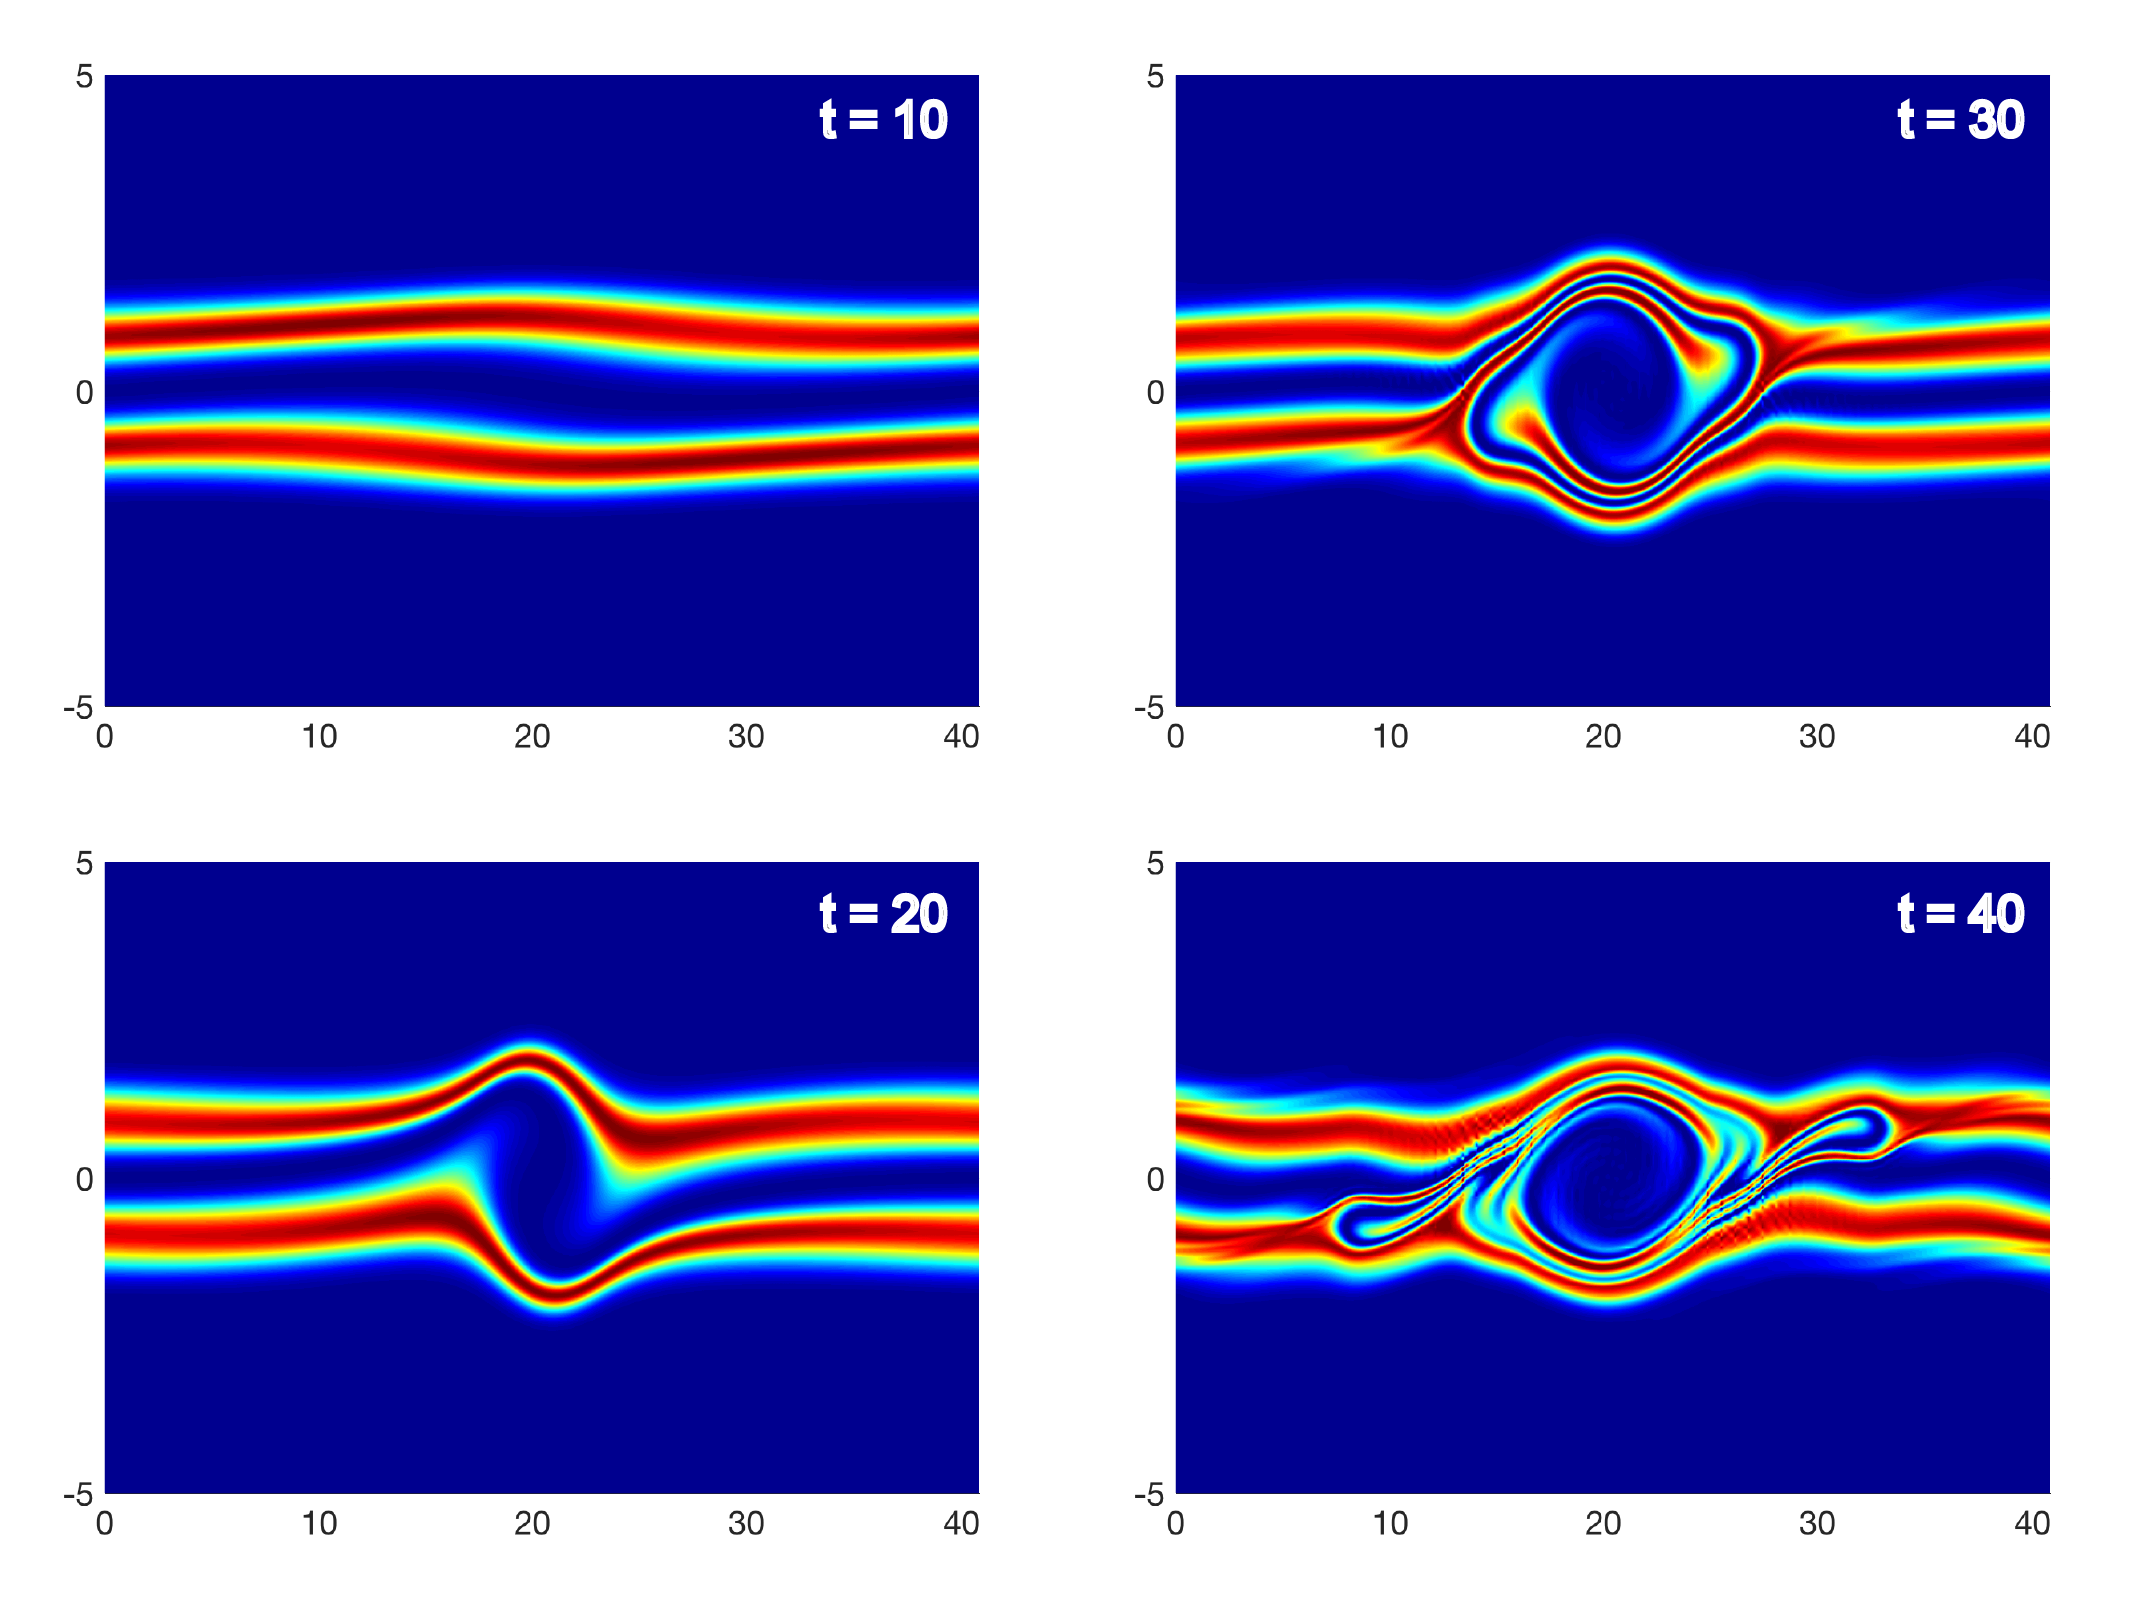
\includegraphics[width=\textwidth]{fp16_fk6d/figures/two-stream-01.png}
    \caption{Phase space ($x$ horizontal, $v$ vertical) contours of the electron probability distribution function $f\left(x,v,t\right)$ as solutions to the two stream instability benchmark at times t=10,20,30,40. These were using the global Lax-Friedrich's choice of numerical flux in the DG method.}
    \label{fig:my_label}
\end{figure}
% Time discretization

% 